\documentclass[12pt]{article}
            \usepackage{sbc-template}
            \makeatletter
            \renewcommand{\inst}[1]{}
            \makeatother
            \usepackage{graphicx,url}
            \usepackage[utf8]{inputenc}
            \usepackage[T1]{fontenc}
            \usepackage[brazil]{babel}
            \usepackage{longtable,booktabs,array}
            \usepackage{amsmath,amssymb}
            \usepackage{fvextra}
            \RecustomVerbatimEnvironment{verbatim}{Verbatim}{%
              breaklines=true,
              breakanywhere=true,
              breaksymbolleft={},
              fontsize=\small
            }
            \providecommand{\tightlist}{%%
              \setlength{\itemsep}{0pt}\setlength{\parskip}{0pt}}
            \providecommand{\pandocbounded}[1]{#1}
            \usepackage{fancyhdr}
            \pagestyle{fancy}
            \fancyhf{}
            \fancyfoot[R]{\thepage}
            \fancyfoot[L]{SANTOS, Anderson F. P. dos — Primeiro pipeline reproduzível}
            \renewcommand{\headrulewidth}{0pt}
            \renewcommand{\footrulewidth}{0.4pt}
            \sloppy
            \title{Primeiro pipeline reproduzível}
            \author{Anderson Fernandes Pereira dos Santos}
            \address{Instituto Militar de Engenharia (IME), Rio de Janeiro, Brazil \\
Venturus Innovation Center, Campinas, Brazil \\
\texttt{anderson@ime.eb.br} | \texttt{anderson.santos@venturus.org.br}}
            \begin{document}

            \maketitle

            \begin{resumo}
            Este artigo transforma a teoria dos dois primeiros capítulos em um pipeline reproduzível de previsão. O objetivo é ensinar o leitor a executar um baseline forte e um primeiro modelo de Reservoir Computing no mesmo recorte adotado no Favorita, medindo ambos com o mesmo protocolo temporal. Fazemos isso em modo passo-a-passo: carregamos a série, separamos treino e teste, executamos \texttt{Seasonal\ Naive}, executamos RC, comparamos previsões, interpretamos métricas e discutimos por que perder para um baseline não invalida um experimento didático. O resultado principal e honesto: no recorte inicial, \texttt{Seasonal\ Naive} supera o RC em todas as métricas, mas o RC funciona de ponta a ponta e abre as perguntas certas para os artigos seguintes.
            \end{resumo}

            \section{O que o leitor vai aprender}\label{1-o-que-o-leitor-vai-aprender}

Ao final deste artigo, você será capaz de:

\begin{enumerate}
\def\labelenumi{\arabic{enumi}.}
\tightlist
\item
  executar um pipeline mínimo de previsão no Favorita;
\item
  usar \texttt{Seasonal\ Naive} como baseline sério, e não apenas ilustrativo;
\item
  rodar o RC clássico do projeto do inicio ao fim;
\item
  comparar previsões com as mesmas métricas e o mesmo split temporal;
\item
  interpretar um resultado inicial ruim como parte do processo científico.
\end{enumerate}

\section{O recorte experimental herdado}\label{2-o-recorte-experimental-herdado}

Continuamos usando exatamente o mesmo recorte estabelecido no artigo 1:

\begin{itemize}
\tightlist
\item
  \texttt{store\_nbr\ =\ 1}
\item
  \texttt{family\ =\ BEVERAGES}
\item
  frequência diária
\item
  últimos \texttt{90} dias como teste
\end{itemize}

Isso significa que a comparação deste artigo e justa por construcao. Ambos os modelos veem os mesmos dados e sao avaliados pelas mesmas métricas.

\section{Passo 1: carregar a série e separar treino e teste}\label{3-passo-1-carregar-a-suxe9rie-e-separar-treino-e-teste}

O pipeline começa com as funções de \texttt{code/common/favorita.py}.

\begin{verbatim}
config = FavoritaSeriesConfig()
frame = load_store_family_series(store_nbr=config.store_nbr, family=config.family)
train, test = temporal_train_test_split(frame, test_days=config.test_days)
\end{verbatim}

Em notação temporal, o experimento usa

\[
\mathcal{D}_{train} = \{(x_t, y_t)\}_{t=1}^{T-90},
\qquad
\mathcal{D}_{test} = \{(x_t, y_t)\}_{t=T-89}^T.
\]

Esse split e fundamental. Se ele mudar entre os modelos, a comparação deixa de ser confiavel.

\section{\texorpdfstring{Passo 2: executar o baseline \texttt{Seasonal\ Naive}}{Passo 2: executar o baseline Seasonal Naive}}\label{4-passo-2-executar-o-baseline-seasonal-naive}

O baseline sazonal do projeto esta em \texttt{code/baselines/seasonal\_naives/model.py} e implementa a regra

\[
\hat{y}_t = y_{t-7},
\]

usando sazonalidade semanal.

A implementação é curta exatamente porque sua função pedagógica e clara:

\begin{verbatim}
pattern = train["y"].to_numpy()[-season_length:]
repeats = int(np.ceil(horizon / season_length))
forecast = np.tile(pattern, repeats)[:horizon]
\end{verbatim}

Para executar:

\begin{verbatim}
python code/baselines/seasonal_naives/run.py
pytest code/baselines/seasonal_naives/test_model.py
\end{verbatim}

Um bom artigo de séries temporais não pula esta etapa. Se um modelo mais sofisticado não supera esse baseline, isso precisa aparecer no texto.

\section{Passo 3: executar o primeiro RC}\label{5-passo-3-executar-o-primeiro-rc}

O RC clássico do projeto esta em \texttt{code/rc/model.py} e usa a configuração default:

\begin{itemize}
\tightlist
\item
  \texttt{n\_reservoir\ =\ 80}
\item
  \texttt{spectral\_radius\ =\ 0.6}
\item
  \texttt{leak\_rate\ =\ 0.15}
\item
  \texttt{washout\ =\ 14}
\end{itemize}

A dinâmica do reservatório é

\[
x_t = (1 - \alpha) x_{t-1} + \alpha \tanh(W_{res} x_{t-1} + W_{in} u_t + b),
\]

e o readout resolve uma regressão Ridge sobre

\[
\phi_t = [1; u_t; x_t].
\]

Para executar:

\begin{verbatim}
python code/rc/run.py
pytest code/rc/test_model.py
\end{verbatim}

\section{Passo 4: medir com o mesmo protocolo}\label{6-passo-4-medir-com-o-mesmo-protocolo}

As quatro métricas usadas na comparação sao:

\[
\mathrm{MAE},\quad \mathrm{RMSE},\quad \mathrm{WAPE},\quad \mathrm{sMAPE}.
\]

O ponto metodológico aqui é simples, mas decisivo: os modelos precisam ser comparados no mesmo horizonte, com as mesmas observações de teste e as mesmas regras de previsão recursiva.

\section{Resultados iniciais}\label{7-resultados-iniciais}

Os resultados reais obtidos no projeto foram os seguintes.

\begin{longtable}[]{@{}lllll@{}}
\toprule\noalign{}
Modelo & MAE & RMSE & WAPE & sMAPE \\
\midrule\noalign{}
\endhead
\bottomrule\noalign{}
\endlastfoot
Seasonal Naive & 259.067 & 352.280 & 0.1196 & 0.1361 \\
RC & 324.294 & 423.417 & 0.1498 & 0.1653 \\
\end{longtable}

O \texttt{Seasonal\ Naive} supera o RC em todas as métricas. Em particular:

\begin{itemize}
\tightlist
\item
  o \texttt{MAE} do RC ficou 25.2\% acima do baseline sazonal;
\item
  o \texttt{RMSE} do RC ficou 20.2\% acima do baseline sazonal.
\end{itemize}

\begin{figure}[htbp]
\centering
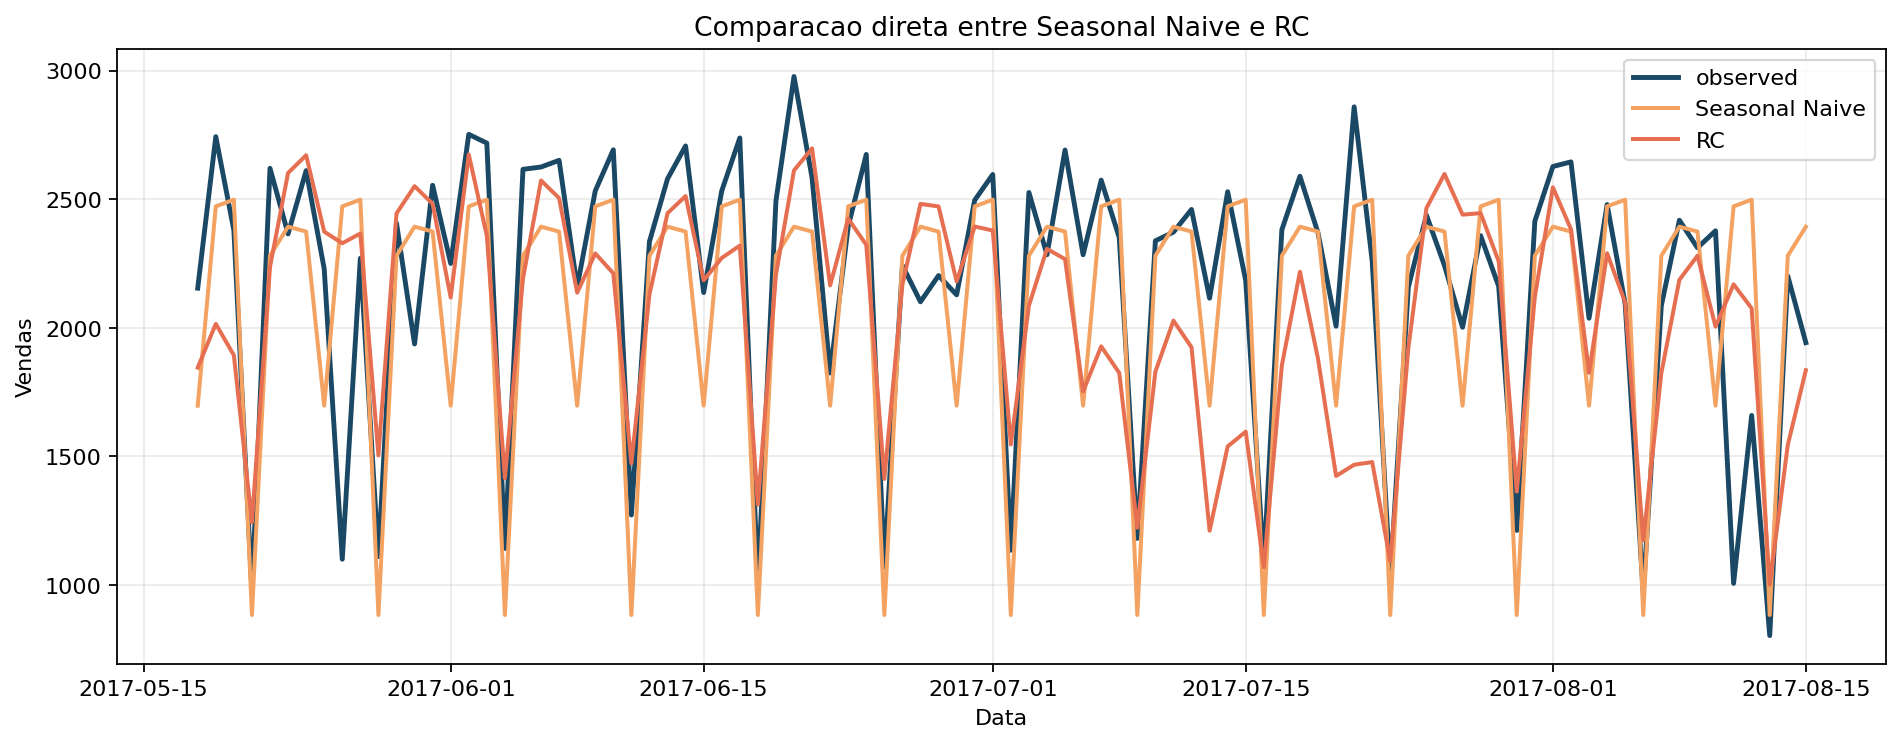
\includegraphics[width=\linewidth,keepaspectratio]{computational_results_20260402_222902/baseline_vs_rc_overlay.png}
\caption{Comparação direta entre o baseline sazonal e o RC no bloco de teste.}
\end{figure}

A sobreposicao das previsões ajuda a ler o resultado com mais cuidado do que a tabela numerica isolada:

\begin{itemize}
\tightlist
\item
  o baseline acompanha melhor o padrão semanal;
\item
  o RC funciona, mas ainda oscila mais em torno da série observada;
\item
  o erro do RC não vem de um colapso do pipeline, e sim de representação insuficiente para este primeiro ajuste.
\end{itemize}

\section{O que este experimento ensina}\label{8-o-que-este-experimento-ensina}

O experimento é didaticamente valioso por quatro motivos.

\subsection{Baseline forte não é detalhe}\label{81-baseline-forte-nuxe3o-uxe9-detalhe}

Em séries temporais, um baseline sazonal simples pode ser surpreendentemente competitivo. Isso vale especialmente quando o sinal semanal e forte, como no caso de bebidas no recorte adotado no Favorita.

\subsection{RC não deve ser tratado como magia}\label{82-rc-nuxe3o-deve-ser-tratado-como-magia}

O RC funciona de ponta a ponta: carrega dados, constroi representação, treina readout e produz previsões. Mas funcionar não é o mesmo que vencer. O artigo faz questão de manter essa distinção.

\subsection{Reprodutibilidade e uma conquista em si}\label{83-reprodutibilidade-e-uma-conquista-em-si}

Este pipeline deixa um trilho completo:

\begin{itemize}
\tightlist
\item
  código de carregamento;
\item
  execucao do baseline;
\item
  execucao do RC;
\item
  testes;
\item
  métricas salvas;
\item
  imagens comparativas.
\end{itemize}

Essa cadeia e o que permite que os artigos seguintes falem de tuning, avaliação justa e QRC sem perder a base experimental.

\subsection{Derrota inicial organiza as próximas perguntas}\label{84-derrota-inicial-organiza-as-pruxf3ximas-perguntas}

Como o RC perdeu para o baseline, os artigos seguintes precisam responder:

\begin{itemize}
\tightlist
\item
  o tamanho do reservatório esta adequado?
\item
  a memória do modelo esta curta ou longa demais?
\item
  o raio espectral esta instável?
\item
  o leak rate esta ajudando ou atrapalhando?
\end{itemize}

Em um bom percurso didático, resultados fracos produzem perguntas fortes.

\section{Como este artigo se conecta ao benchmark maior}\label{9-como-este-artigo-se-conecta-ao-benchmark-maior}

O experimento deste artigo não encerra a comparação. Ele apenas estabelece o primeiro patamar:

\begin{itemize}
\tightlist
\item
  \texttt{Seasonal\ Naive} será mantido como referencia;
\item
  RC será refinado e estudado com mais detalhe;
\item
  novos competidores entrarao depois: \texttt{ETS}, \texttt{Prophet}, \texttt{XGBoost}, \texttt{LSTM} e \texttt{QRC}.
\end{itemize}

Essa progressao e importante porque impede um salto artificial do "primeiro RC" diretamente para o "QRC final".

\section{Conclusão}\label{10-conclusuxe3o}

O primeiro pipeline reproduzível da série esta fechado. O baseline sazonal venceu, o RC funcionou sem vencer e o leitor já tem um experimento concreto para estudar, modificar e rerodar. Isso é exatamente o que um artigo didático deveria entregar neste ponto: menos promessas vagas e mais reprodução concreta.

O próximo artigo vai usar essa base para explicar por que RC pode melhorar ou piorar tanto quando seus hiperparâmetros mudam.

\section*{Entregaveis associados no repositorio}\label{entregaveis-associados-no-repositorio}

\begin{itemize}
\tightlist
\item
  baseline sazonal: \texttt{code/baselines/seasonal\_naives/}
\item
  RC clássico: \texttt{code/rc/}
\item
  comparação numerica e visual deste artigo: \texttt{computational\_results\_20260402\_222902/}
\item
  figuras principais: \texttt{baseline\_vs\_rc\_overlay.png}, \texttt{seasonal\_naive\_forecast\_plot.png}, \texttt{rc\_forecast\_plot.png}
\end{itemize}

\section{Referências}\label{referencias}

\begin{thebibliography}{9}

\bibitem{jaeger2001}
JAEGER, H. \textbf{The ``echo state'' approach to analysing and training recurrent neural networks}. Bonn: German National Research Center for Information Technology (GMD), 2001.

\bibitem{lukosevicius2009}
LUKOSEVICIUS, M.; JAEGER, H. \textbf{Reservoir computing approaches to recurrent neural network training}. \emph{Computer Science Review}, v. 3, n. 3, p. 127--149, 2009.

\bibitem{lukosevicius2012}
LUKOSEVICIUS, M. \textbf{A practical guide to applying echo state networks}. In: MONTAVON, G.; ORR, G. B.; MÜLLER, K.-R. (org.). \emph{Neural Networks: Tricks of the Trade}. 2. ed. Berlin: Springer, 2012. p. 659--686.

\bibitem{fujii2017}
FUJII, K.; NAKAJIMA, K. \textbf{Harnessing disordered-ensemble quantum dynamics for machine learning}. \emph{Physical Review Applied}, v. 8, n. 2, 024030, 2017.

\end{thebibliography}

            \end{document}
